\begin{answer}


All picture wrt $\tau$ = [0.03, 0.05, 0.1, 0.5, 1, 10] has attach with corresponding names.


best $\tau$ = 0.05, MSE on the test split using this $\tau$ value is 0.016906174581478528

\begin{figure}
    \centering
    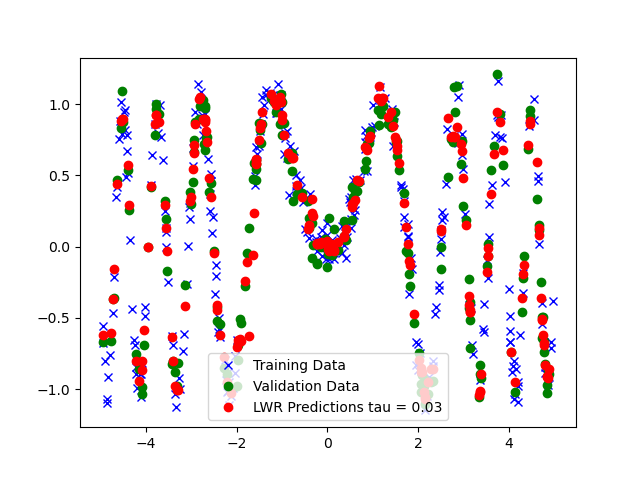
\includegraphics[width=0.5\linewidth]{ps1_q2_(c)_tau_0.03.png}
    \caption{ps1\_q2\_(c)\_tau\_0.03}
    \label{fig:enter-label}
\end{figure}

\begin{figure}
    \centering
    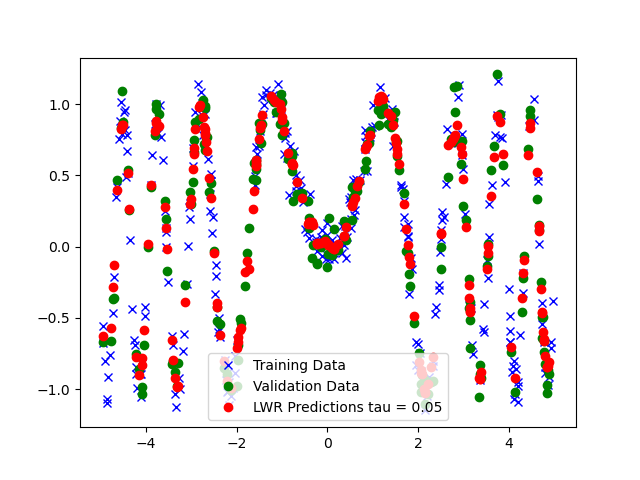
\includegraphics[width=0.5\linewidth]{ps1_q2_(c)_tau_0.05.png}
    \caption{ps1\_q2\_(c)\_tau\_0.05}
    \label{fig:enter-label}
\end{figure}

\begin{figure}
    \centering
    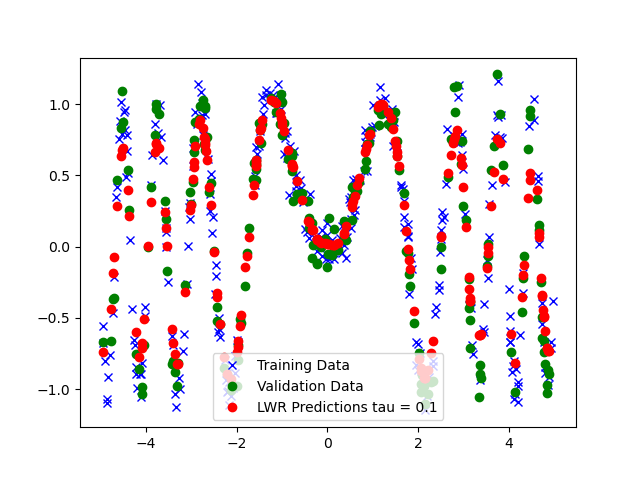
\includegraphics[width=0.5\linewidth]{ps1_q2_(c)_tau_0.1.png}
    \caption{ps1\_q2\_(c)\_tau\_0.1}
    \label{fig:enter-label}
\end{figure}

\begin{figure}
    \centering
    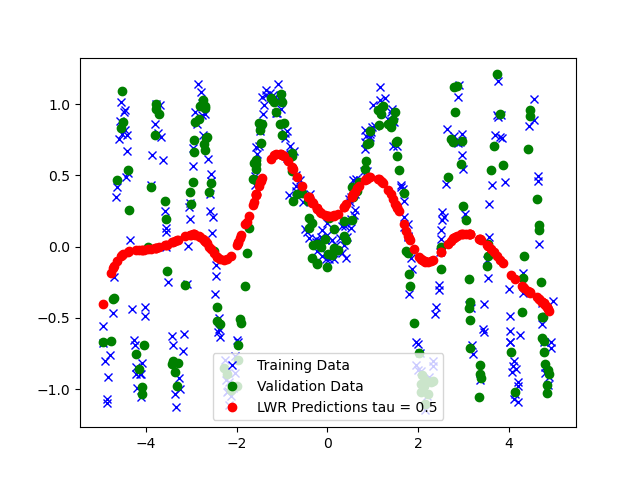
\includegraphics[width=0.5\linewidth]{ps1_q2_(c)_tau_0.5.png}
    \caption{ps1\_q2\_(c)\_tau\_0.5}
    \label{fig:enter-label}
\end{figure}

\begin{figure}
    \centering
    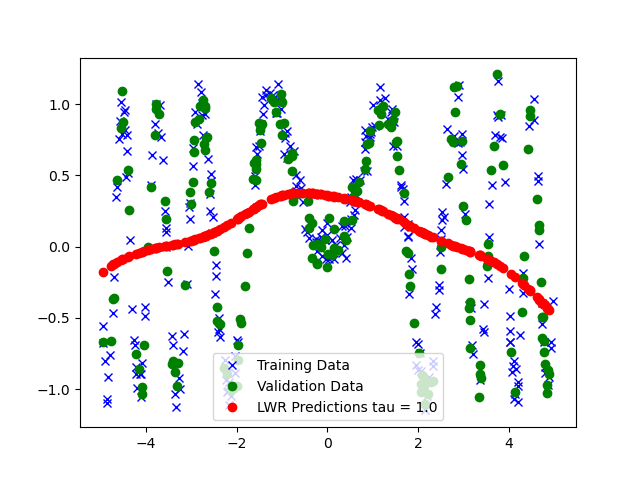
\includegraphics[width=0.5\linewidth]{ps1_q2_(c)_tau_1.0.png}
    \caption{ps1\_q2\_(c)\_tau\_1}
    \label{fig:enter-label}
\end{figure}

\begin{figure}
    \centering
    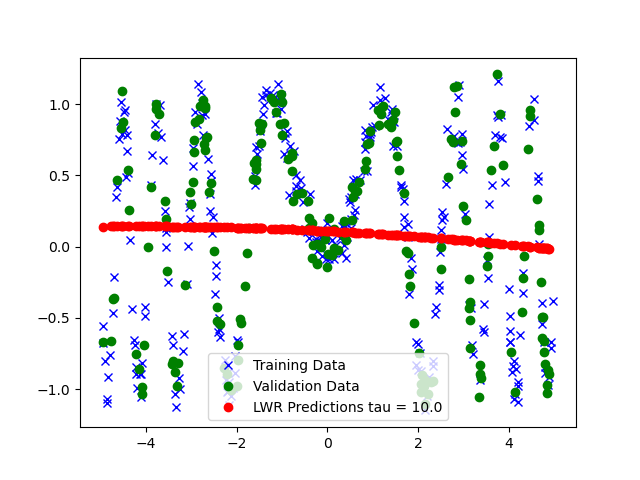
\includegraphics[width=0.5\linewidth]{ps1_q2_(c)_tau_10.0.png}
    \caption{ps1\_q2\_(c)\_tau\_10}
    \label{fig:enter-label}
\end{figure}
\end{answer}
